To test the processor we did several things. First we did a reverse string test, then a Fibbonaci program and lastly a Pong game. The reverse string and the Fibbonaci programs were outputted via the serial. The Pong game had input from a computer keyboard via a serial cable to control the flipper, a ball that was flying around with edge detection and VGA output to show the game on a computer screen. 

\begin{figure}[!h]
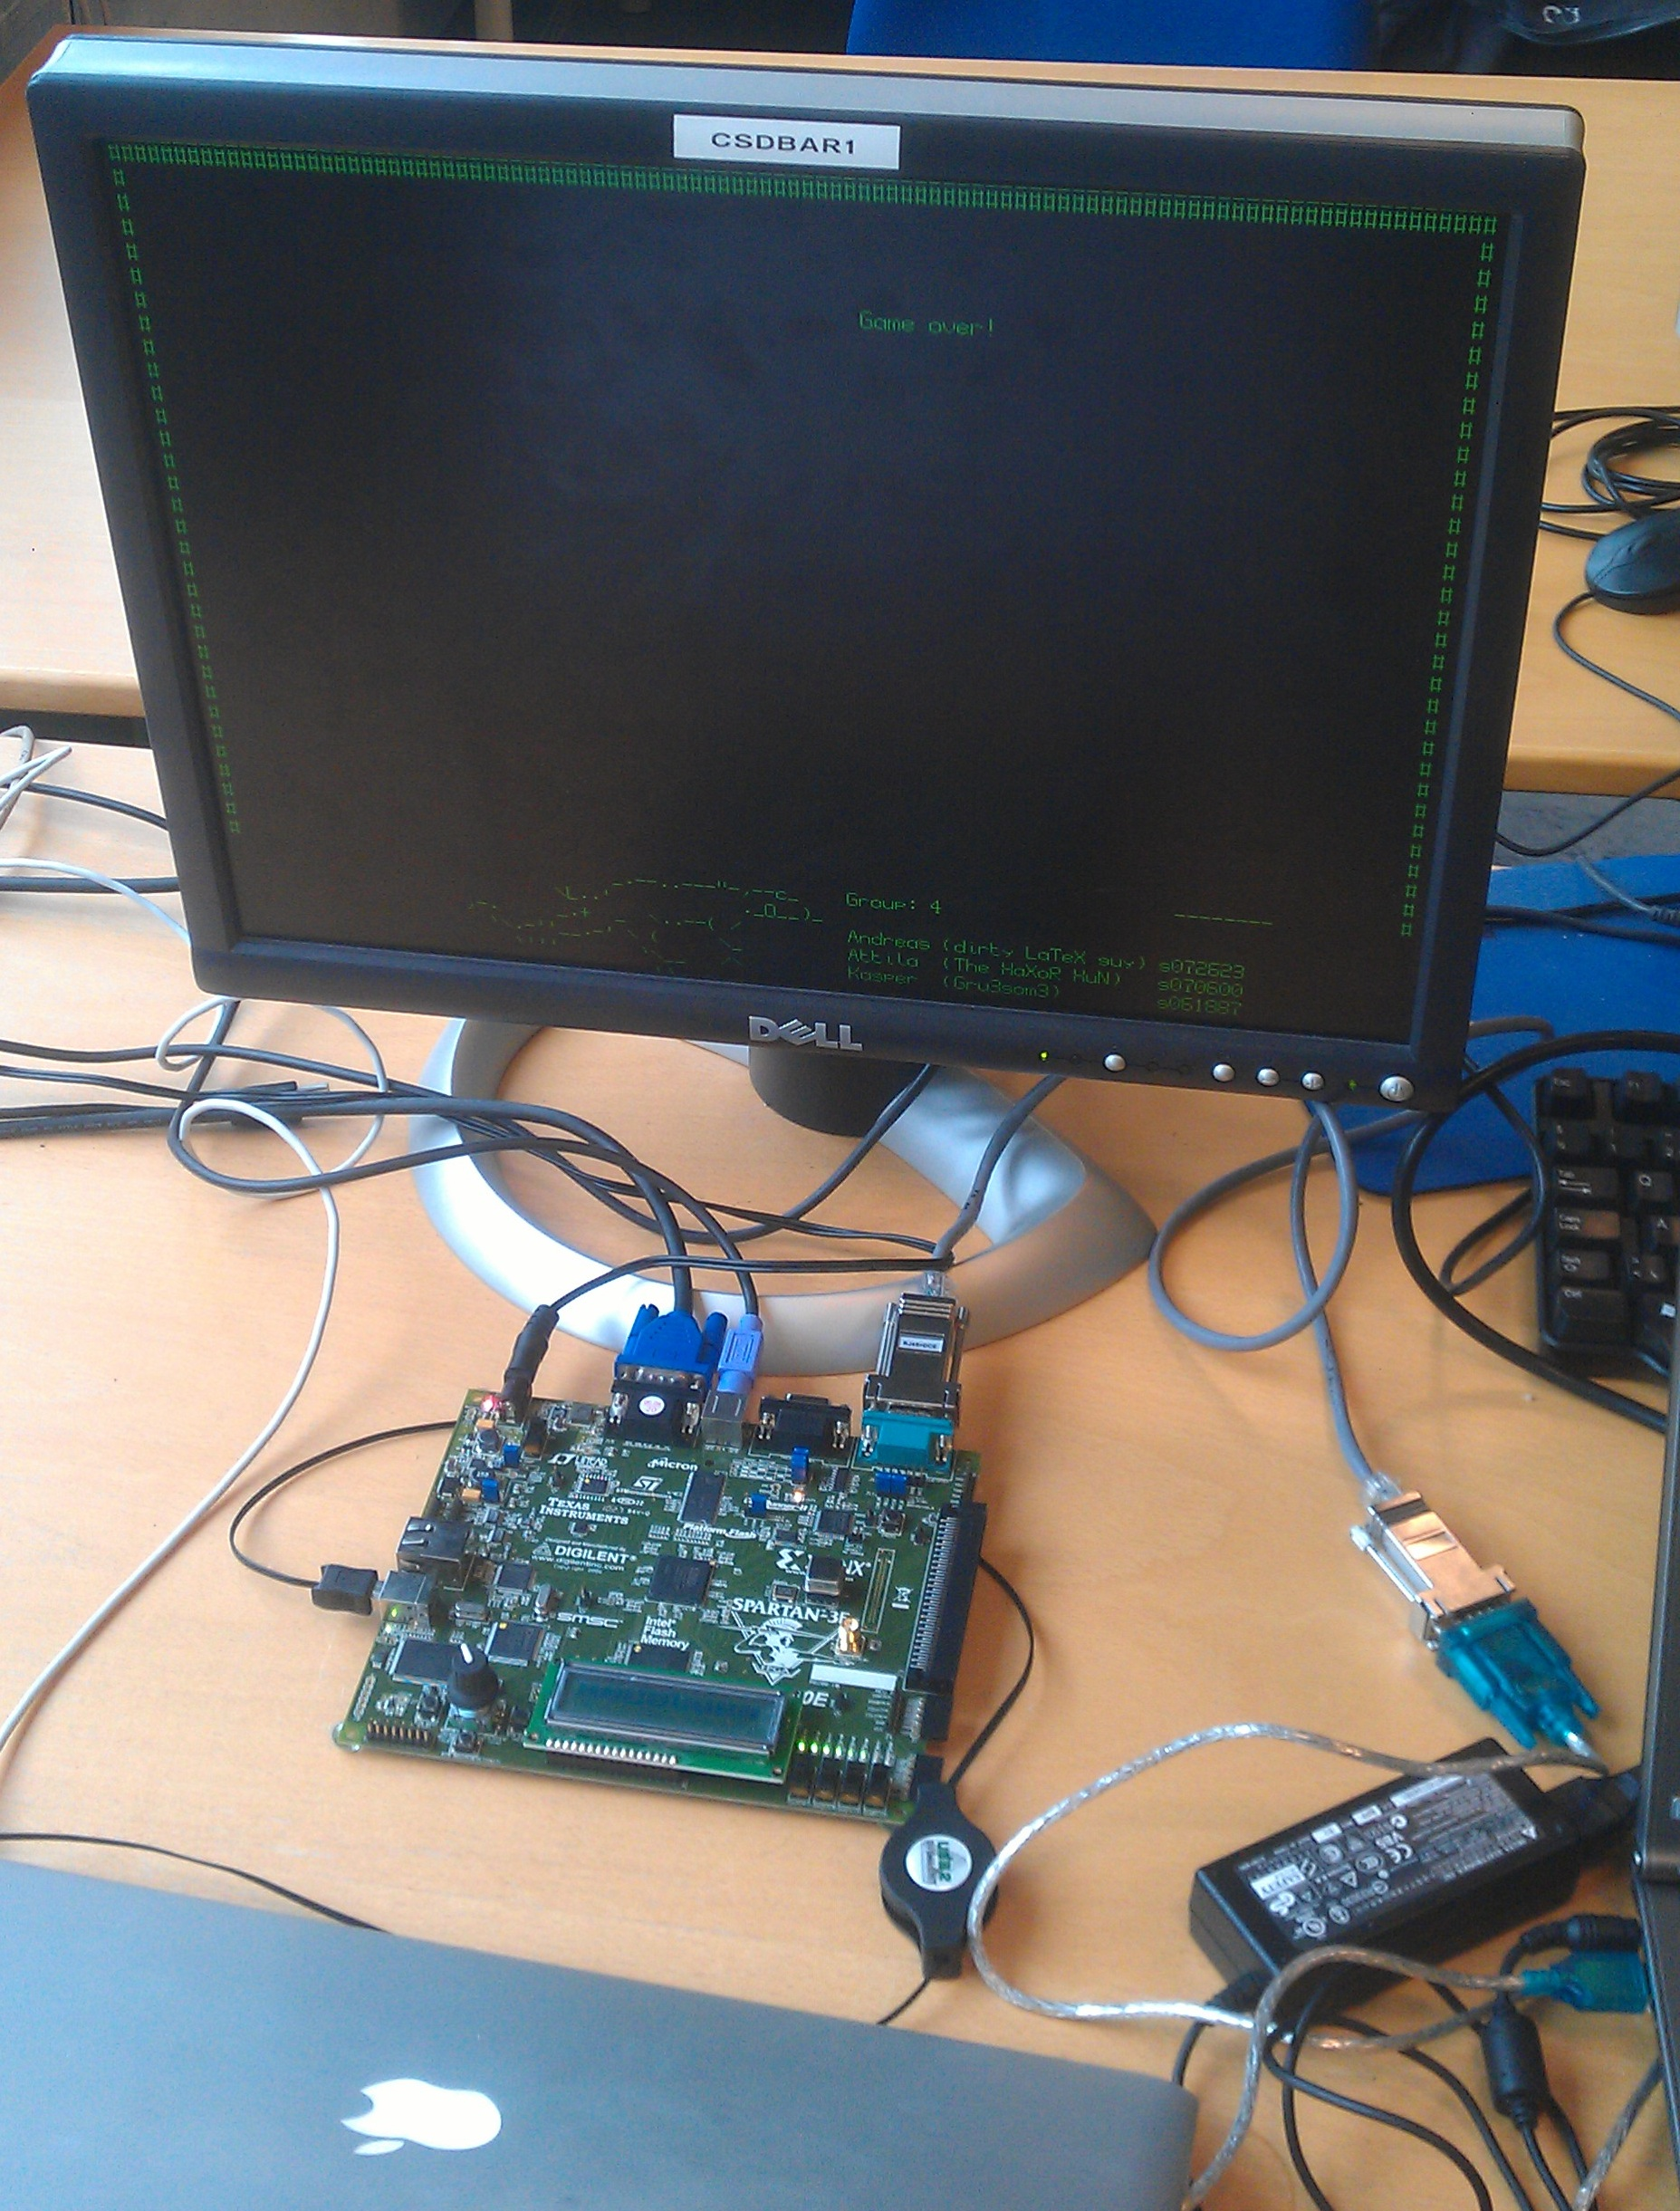
\includegraphics[width=0.45\textwidth]{Images/pong.jpg}
\caption{The pong game running on the MIPS on the FPGA.}
\label{fig:pong}
\end{figure}

As the programs grew in complexity our processor still managed to run them. In the Pong game we reached over a thousand lines of assembler code. Since we didn't implement all the functionalities in the MIPS processor, we sometime had to manually change some MIPS instructions to get the C program to work. However, with the implemented instructions, all MIPS core instructions could be emulated as pseudo instructions.

